\thispagestyle{fancy}
\chapter{System Interface} \label{ch:system_interface}
\section*{\centering Chapter \thechapter}
\section*{\centering System Interface}

The system takes data in CSV format. A web-based GUI will be offered to users. We are using a flask-based web app for easier integration of the main system. We have implemented separate pages for users depending on tasks. These pages are the selection page, prediction page, performance page, and cross-performance page. We will see a detailed explanation of the pages and the process carried out in the background.

\section{System Design} \label{sec:system_design}

The server is accessed with the help of a port number. The site is accessed by URL in the form of \url{http://ip_address:port_number} URL syntax. In this development server we are using \url{http} protocol and \url{127.0.0.1} or \url{localhost} as \url{ip_address}. The \url{port_number} \url{5000} is used as per flask recommendation. Hence, the URL used by the application to access the website is \url{http://localhost:5000}. In the next subsections, we will go through each page available to the user.

\subsection{Login Page} \label{subsec:login_page}
This page is the first page encountered by a user when logging on to the website. This page will take a valid username and password from the user and start the session for that username. After starting the session, the user will be redirected to the Home page. \Cref{fig:web_login_page} displays the login page.

\begin{figure}[H]
  \centering
  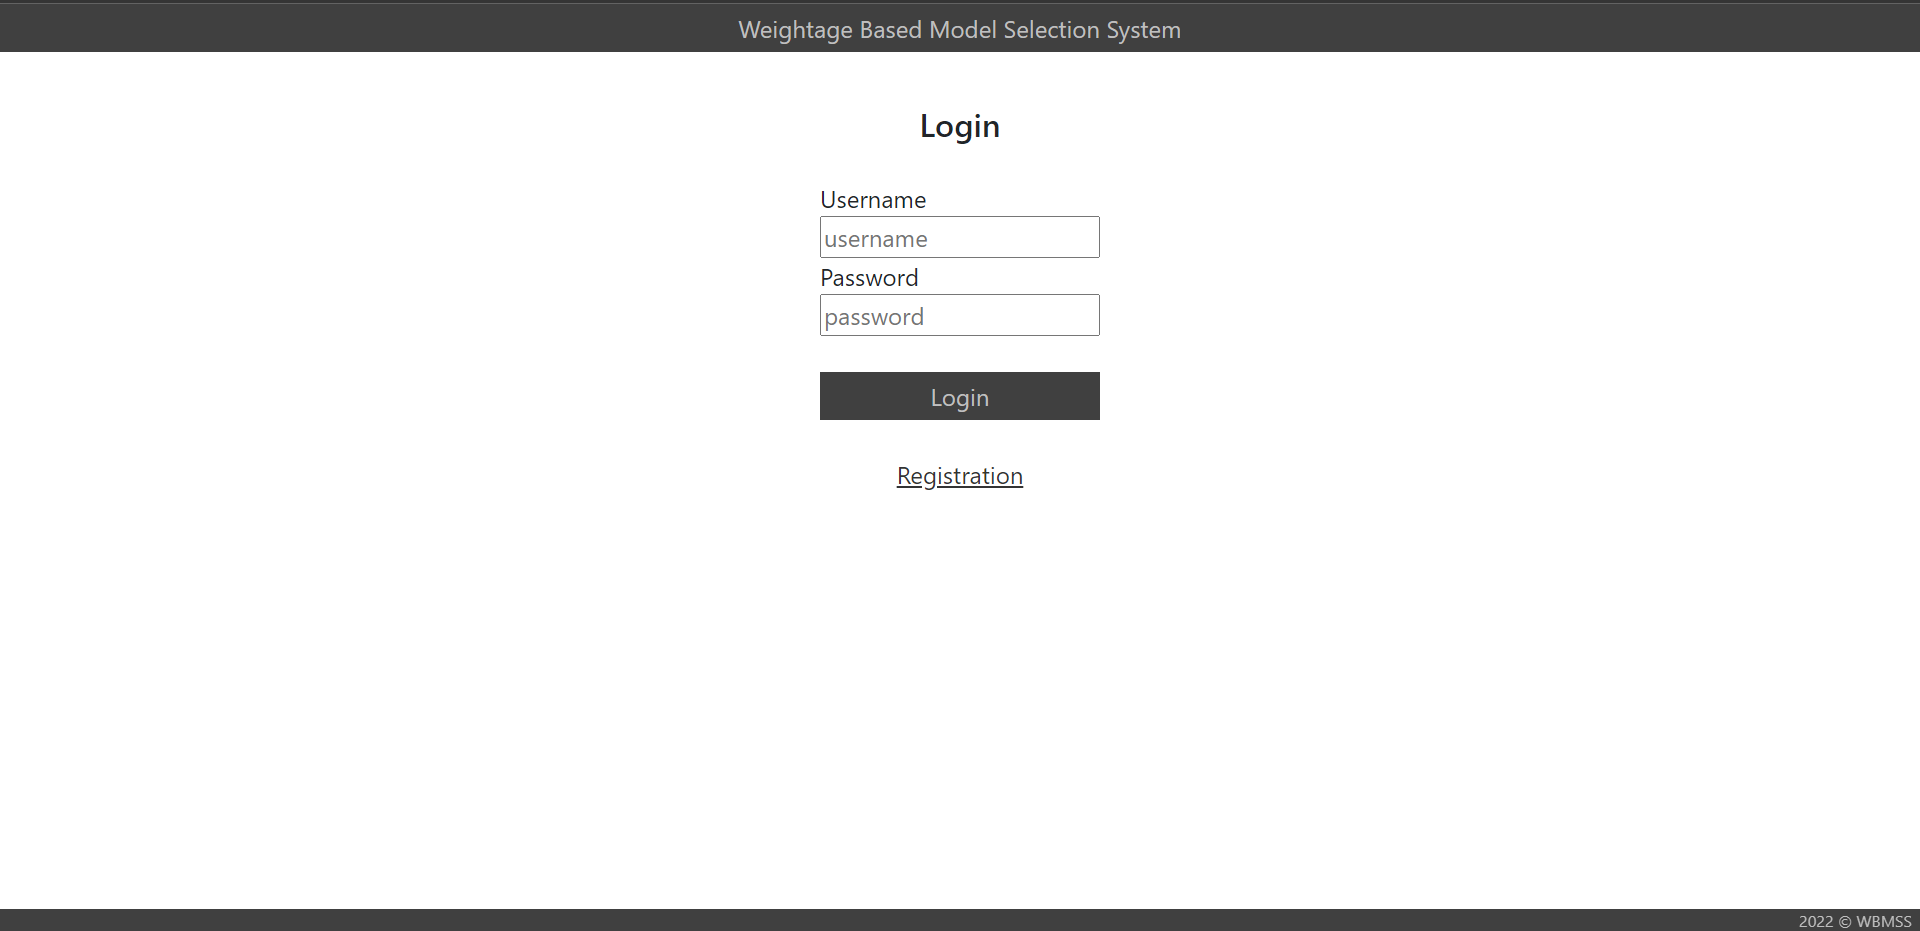
\includegraphics[width=0.7\columnwidth]{media/website/pages/login.png}
  \caption{Login Page}
  \label{fig:web_login_page}
\end{figure}

\subsection{Home Page} \label{subsec:home_page}
The home page is the landing page for the users after the session is started. It provides information about the website. The side navigation is provided for users for easier access to the rest of the website. This side navigation is present on all the pages except the login page.

\begin{figure}[H]
  \centering
  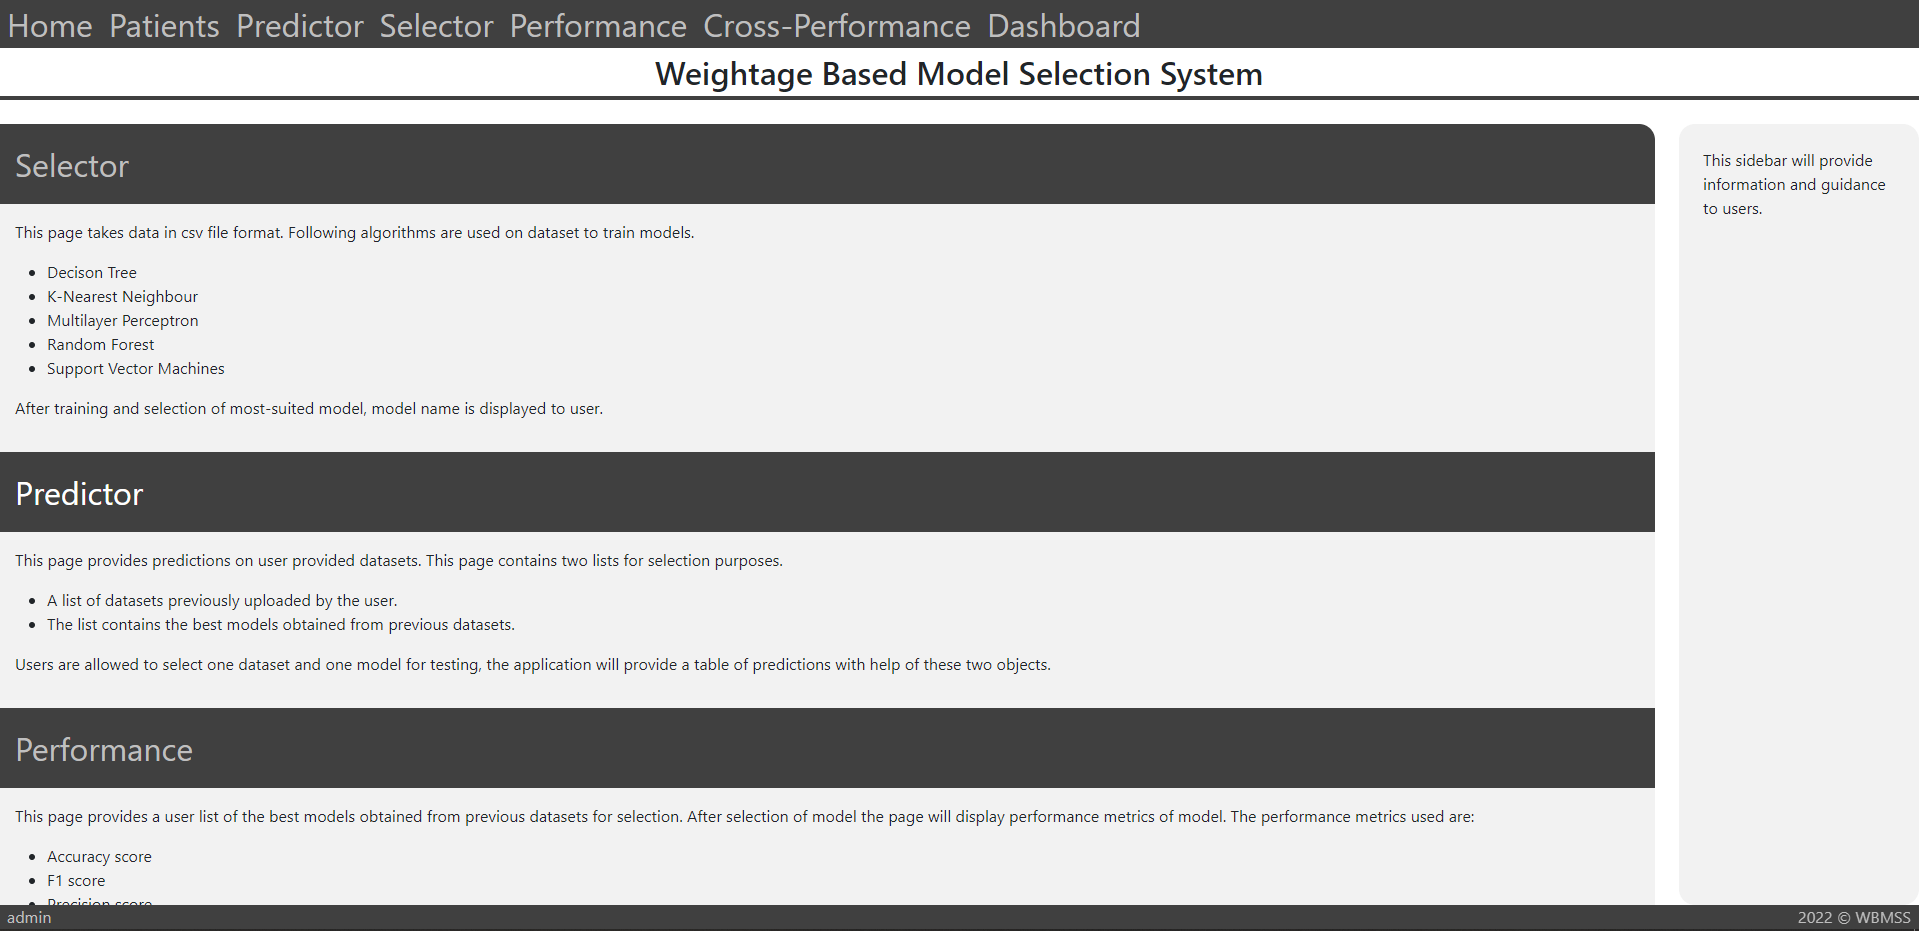
\includegraphics[width=0.7\columnwidth]{media/website/pages/home.png}
  \caption{Home Page}
  \label{fig:home_page}
\end{figure}

\FloatBarrier
\subsection{Selector Page} \label{subsec:selector_page}
This page takes file input from the user. Currently, only CSV file format is supported. The files are copied into the directory of the application. The training and selection module will process the copied file. These modules will execute model training, performance evaluation, and selection process. After process completion, the user will receive confirmation. \Cref{fig:web_selector_page} displays the selector page.

\begin{figure}[H]
  \centering
  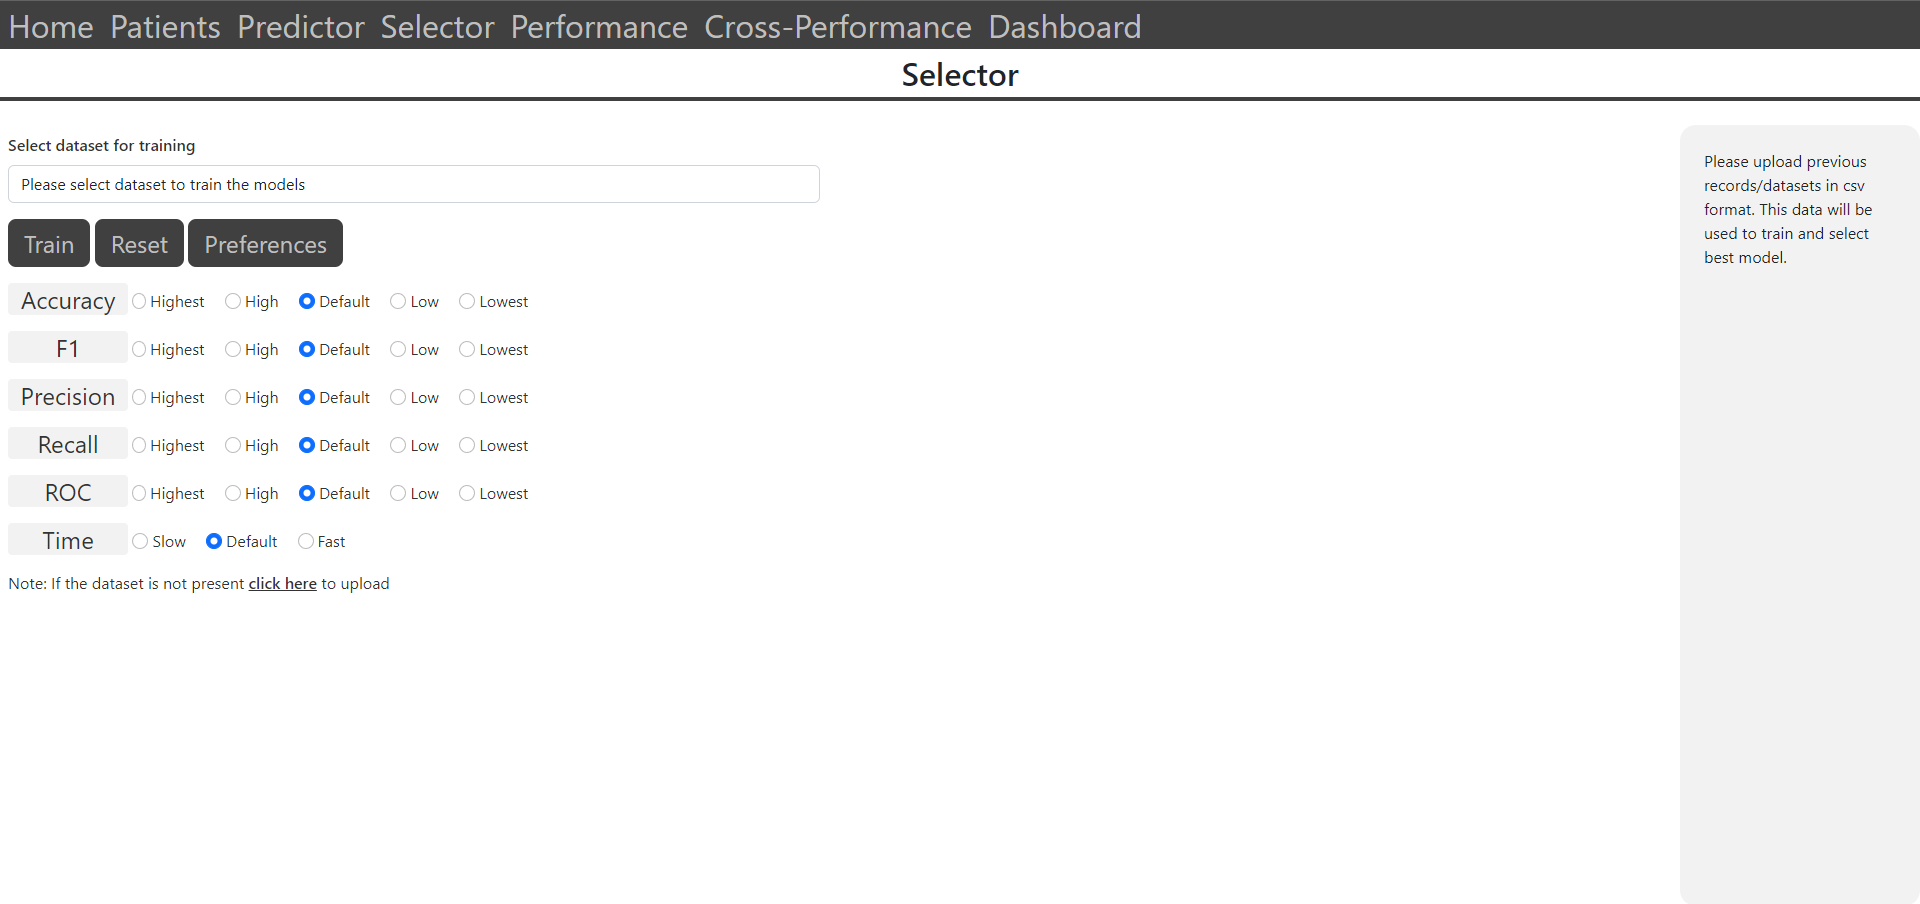
\includegraphics[width=0.7\columnwidth]{media/website/pages/selector.png}
  \caption{Selector Page}
  \label{fig:web_selector_page}
\end{figure}

\subsubsection{Display Selected Model Page} \label{subsec:display_selected_model_page}
This page is a subpage to the selector page. This page is used to display the name of the selected classifier to the user. This page has a similar layout to the selector page with a small difference, and it acts similarly to the selector page. \Cref{fig:display_selected_model_page} displays the selector-upload subpage.

\begin{figure}[H]
  \centering
  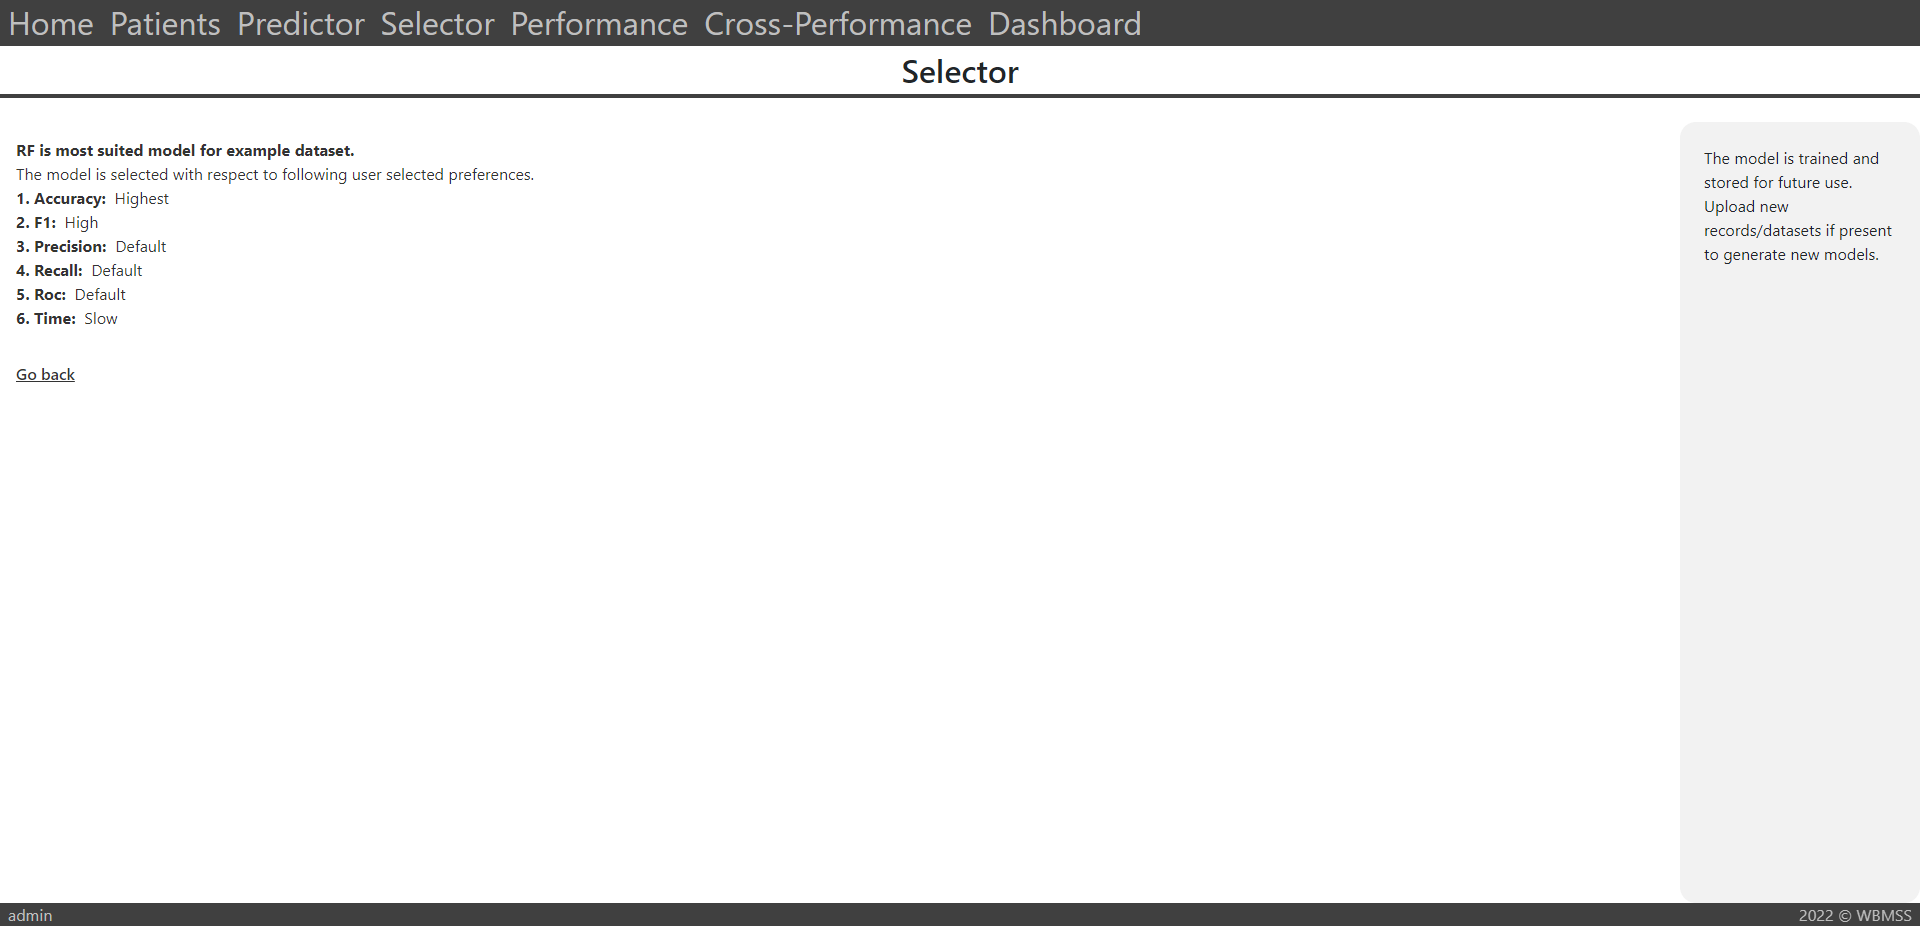
\includegraphics[width=0.7\columnwidth]{media/website/pages/selector_selected.png}
  \caption{Display Selected Model Page}
  \label{fig:display_selected_model_page}
\end{figure}

\subsection{Patients Page}\label{subsec:patients_page}
This consist of two subpages 1. registration page and 2. reports page. The registartion page generates user registration form and accepts values from logged user. \Cref{fig:patient_registration_page} shows the registration form. The reports page provides user a list of patinets, as shown in \cref{fig:patient_selection_page}. The result of selected patient is displayed along with link to his ECG report, as shown in \cref{fig:patients_report}.

\begin{figure}
  \centering
  \begin{subfigure}{.7\columnwidth}
    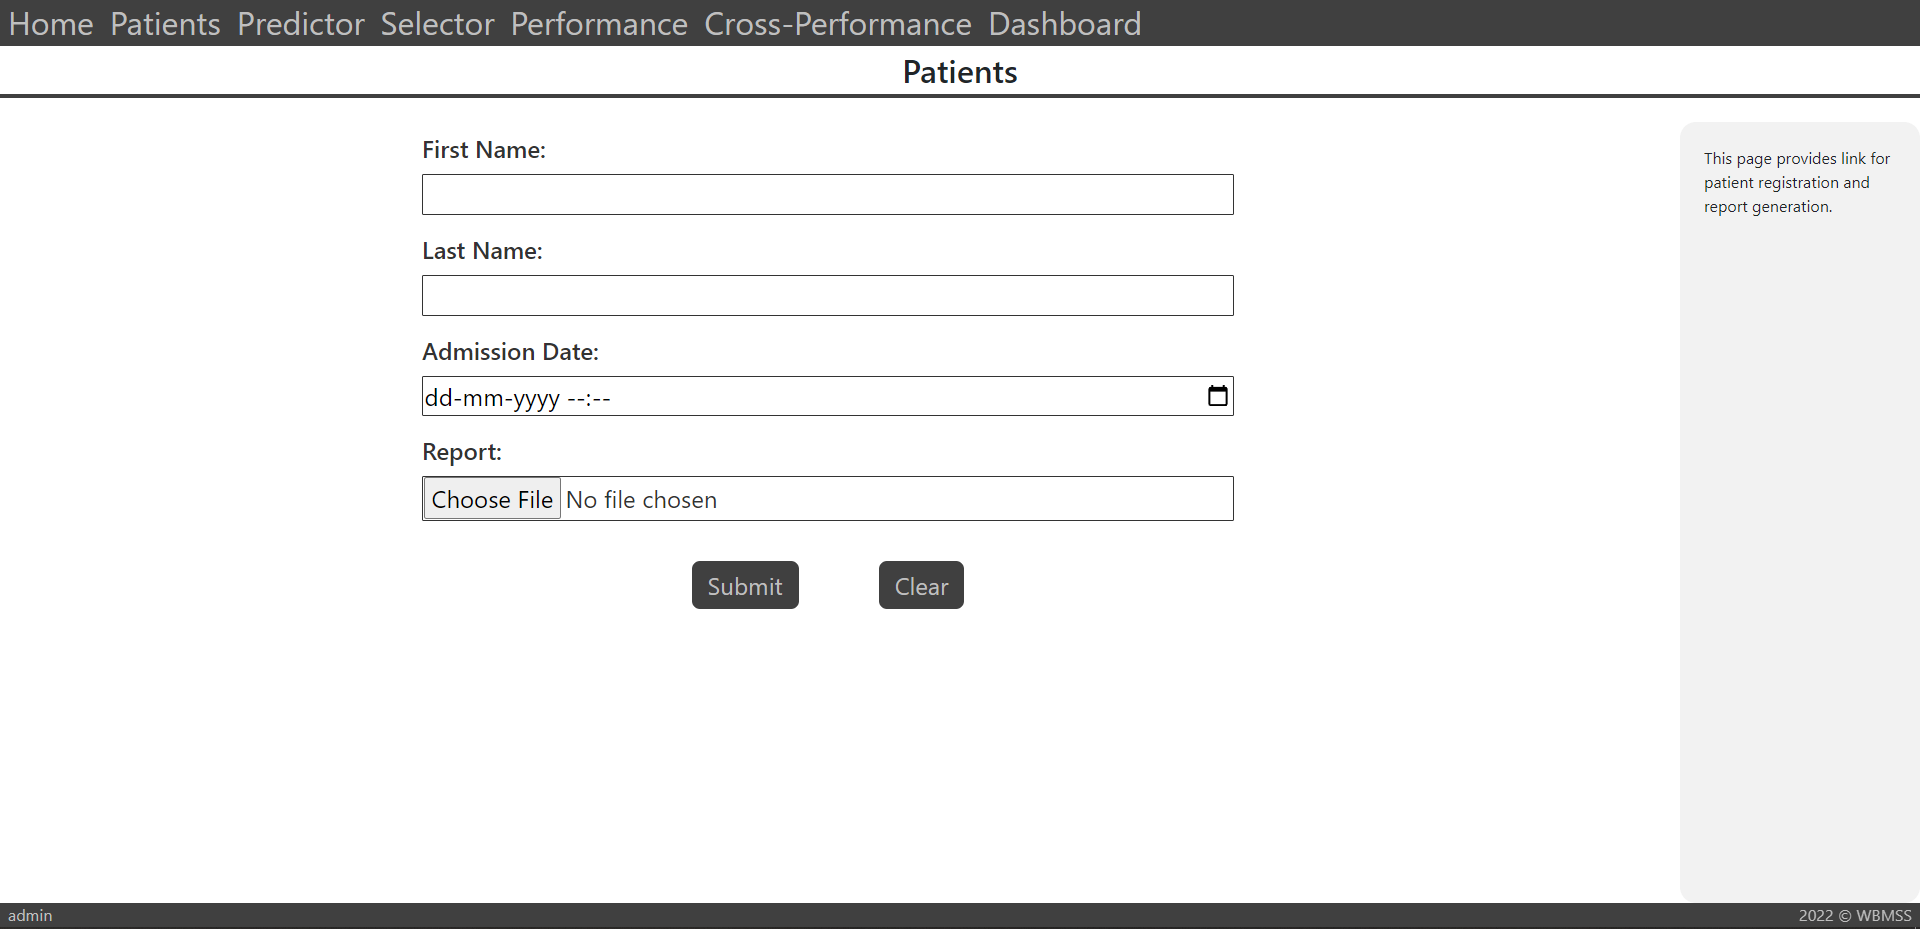
\includegraphics[width=\columnwidth]{media/website/pages/registration.png}
    \caption{Patient Registration Page}\label{fig:patient_registration_page}
  \end{subfigure}
  \begin{subfigure}{.7\columnwidth}
    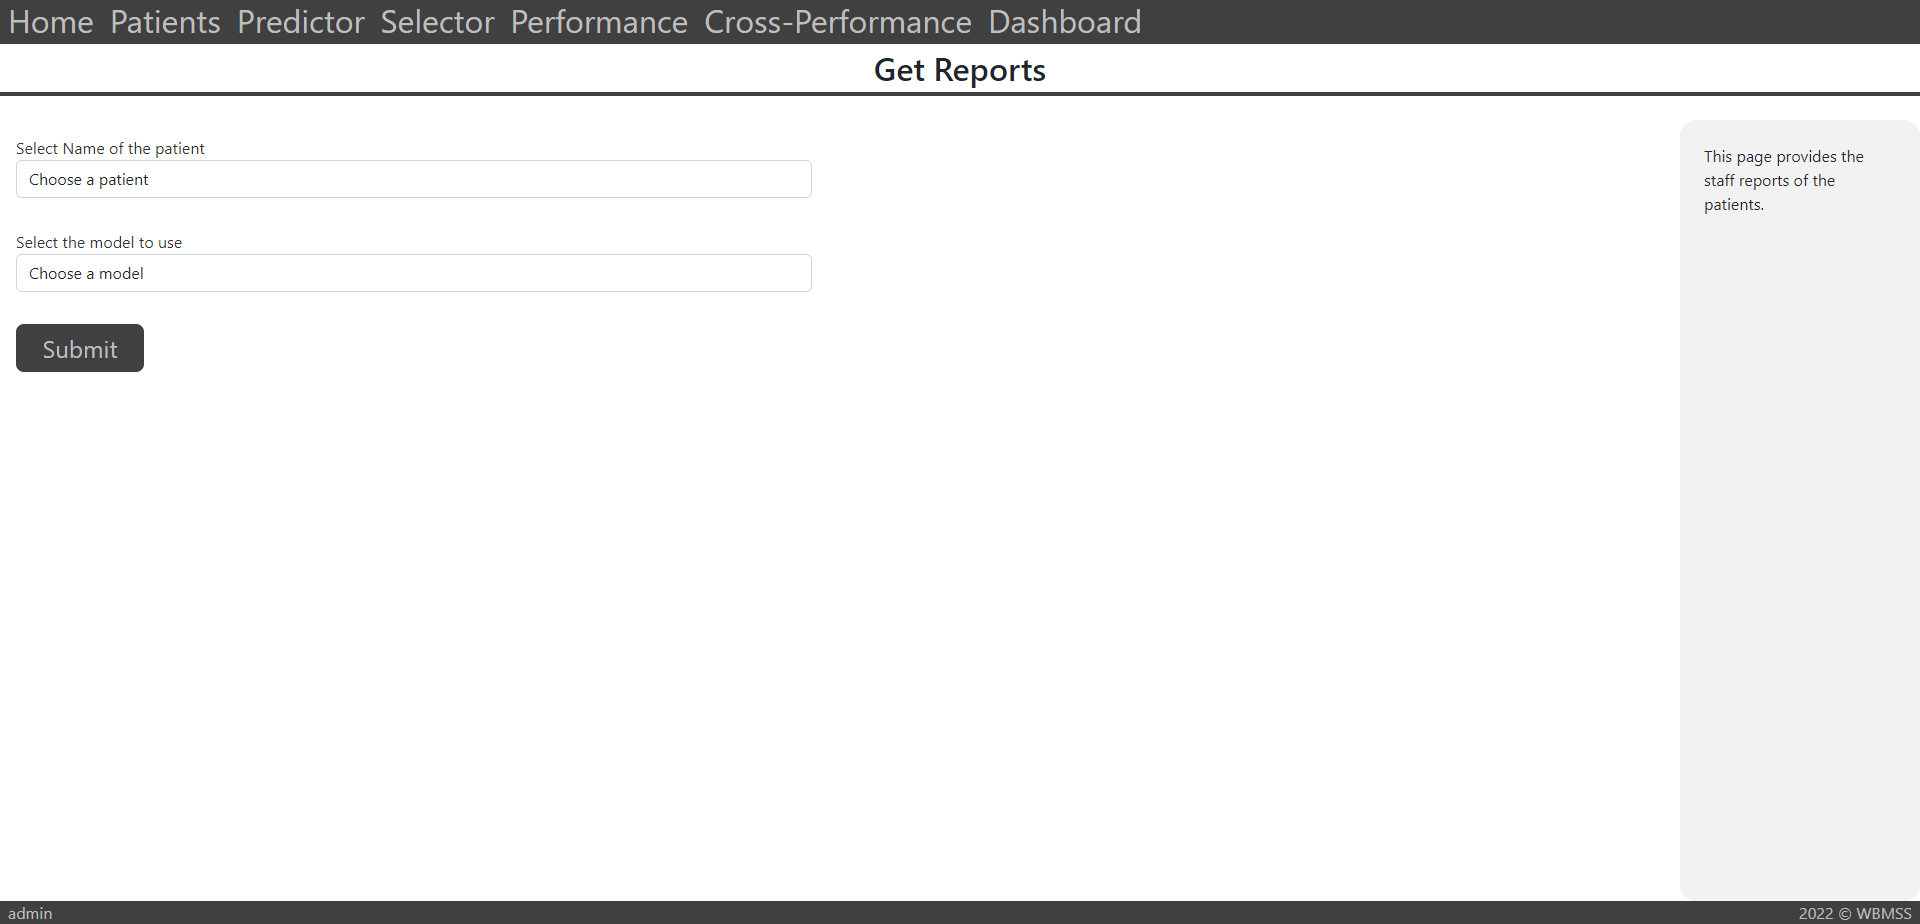
\includegraphics[width=\columnwidth]{media/website/pages/get_report.png}
    \caption{Patient Selection Page}\label{fig:patient_selection_page}
  \end{subfigure} \\
  \begin{subfigure}{.7\columnwidth}
    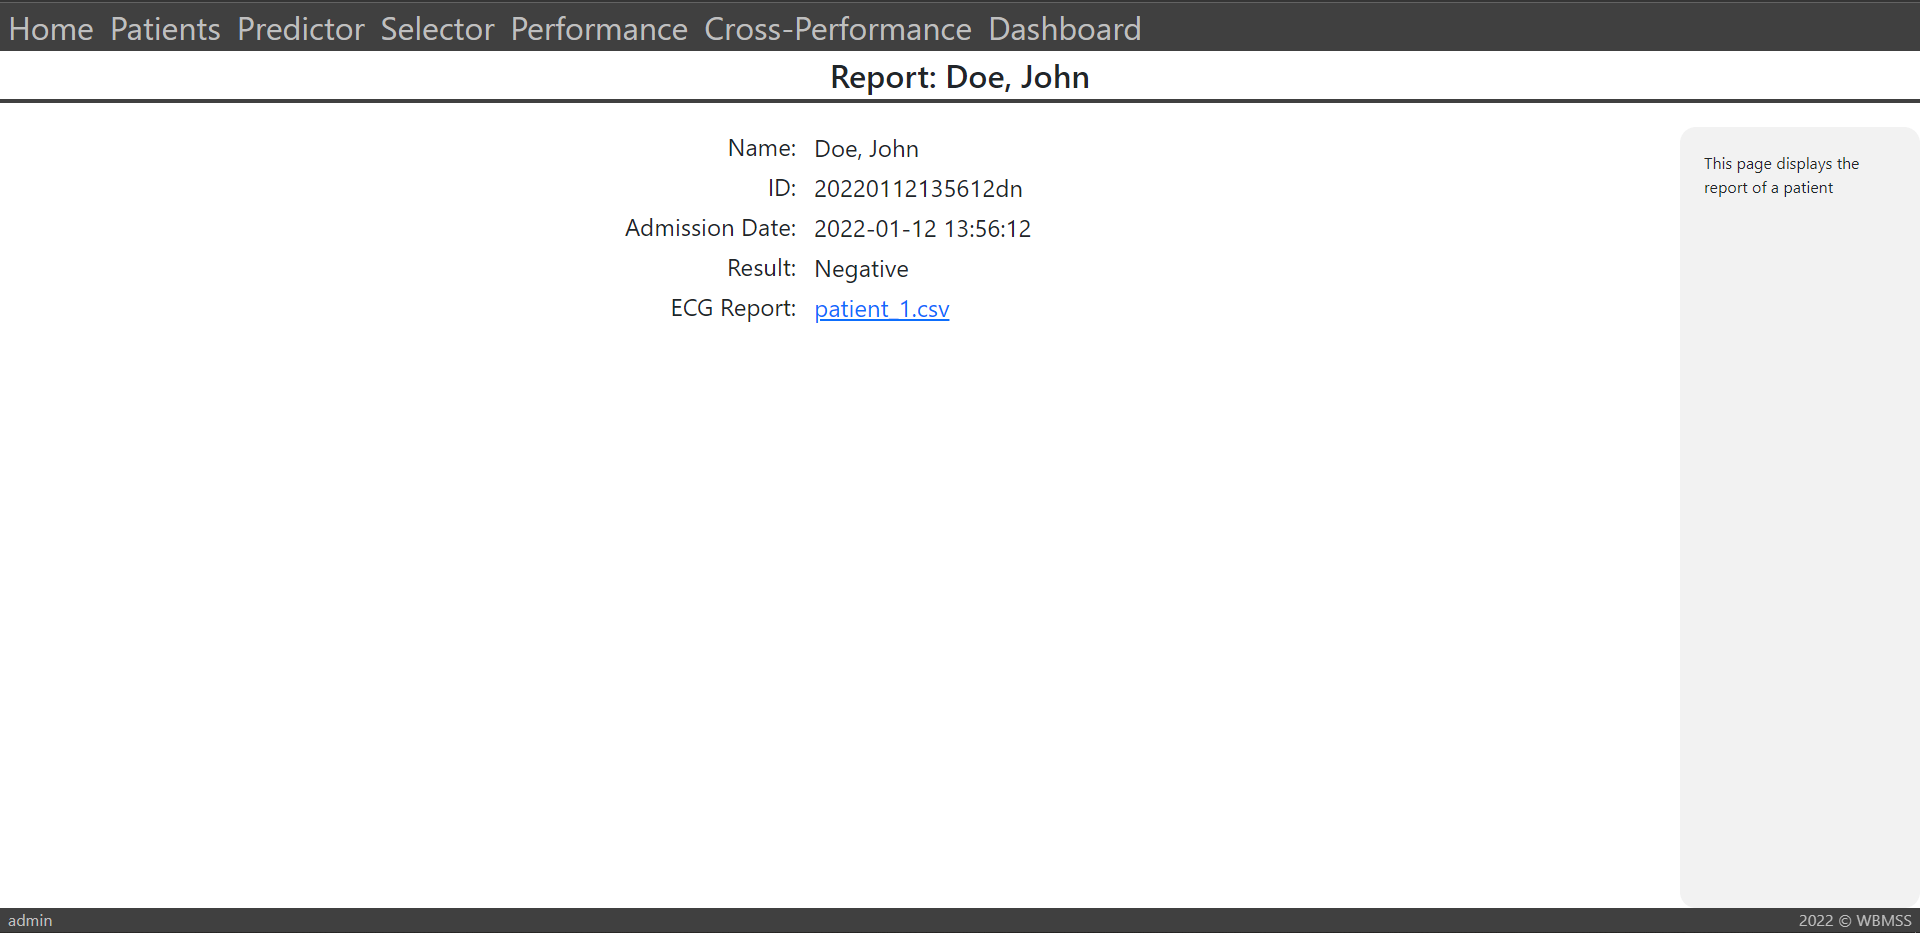
\includegraphics[width=\columnwidth]{media/website/pages/get_report_display.png}
    \caption{Patients Report}\label{fig:patients_report}
  \end{subfigure}
  \caption{Patients Pages}\label{fig:patients_page}
\end{figure}

\FloatBarrier
\subsection{Predictor Page} \label{subsec:predictor_page}
This page is used to make predictions based on the dataset provided by the user. This page generates a list of the best models for users to select models for predictions. The page also generated a list of datasets provided by the user for predictions. If the dataset is not available, the user is allowed to upload the dataset from the page. After submitting the selected model and dataset page will run the prediction process on the datasets. After completion of this process, the user is forwarded to the subpage. \Cref{fig:web_predictor_page} displays the predictor page.

\begin{figure}[H]
  \centering
  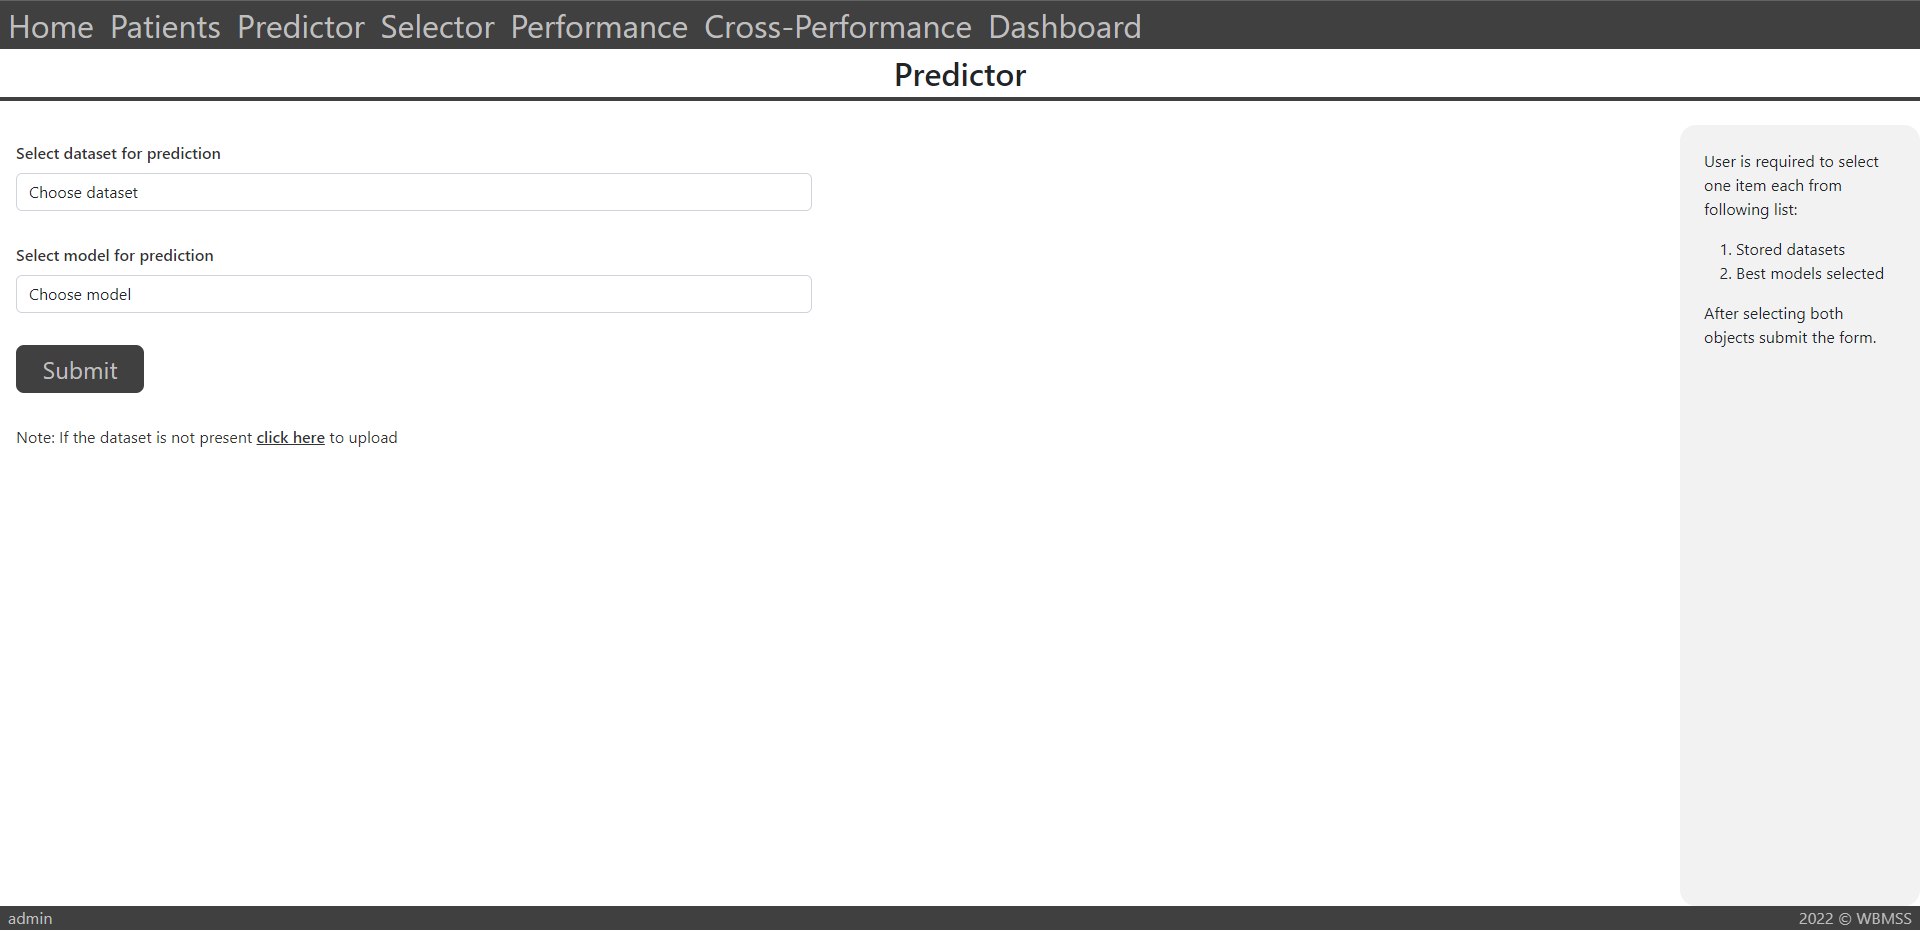
\includegraphics[width=0.7\columnwidth]{media/website/pages/predictor.png}
  \caption{Predictor Page}
  \label{fig:web_predictor_page}
\end{figure}

\subsubsection{Predictor Results Page} \label{subsubsec:predictor_result_page}
This page will display the results of predictions obtained from the model and dataset submitted by the user with the predictor page. The result is displayed in tabular format with ID and prediction results as columns. \Cref{fig:web_predictor_results_page} displays the predictor-results subpage.

\begin{figure}[H]
  \centering
  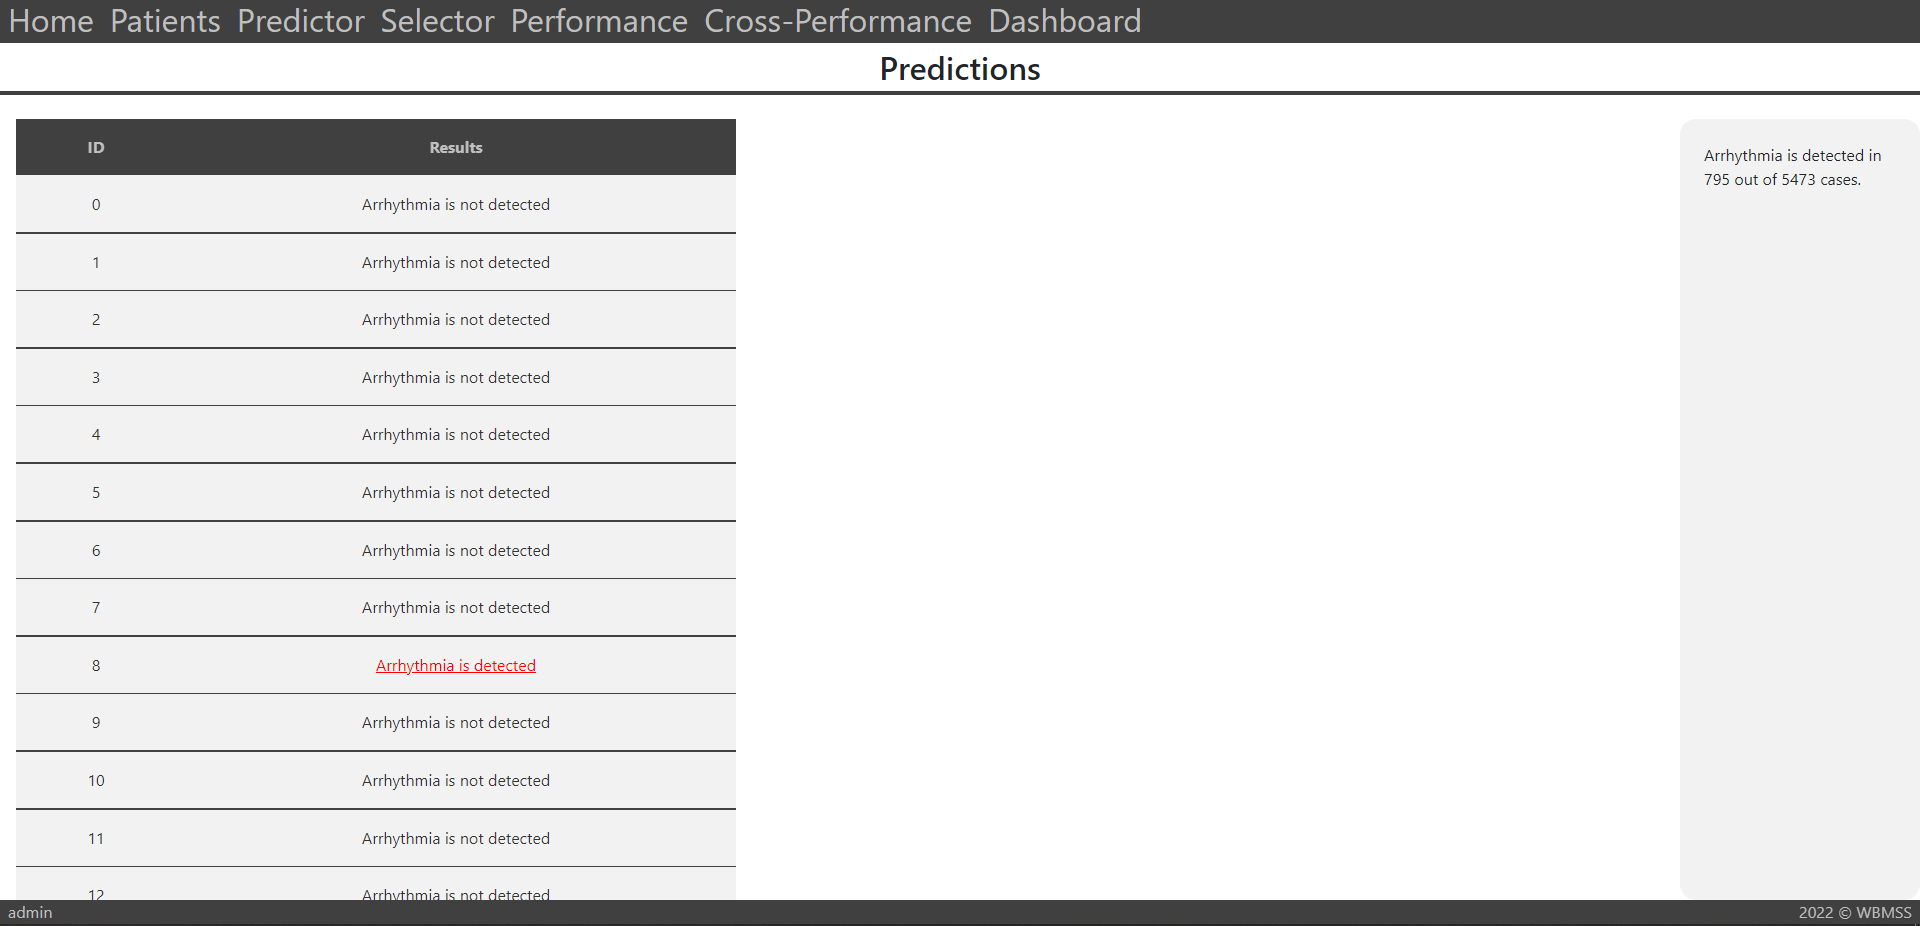
\includegraphics[width=0.7\columnwidth]{media/website/pages/predictor_display.png}
  \caption{Predictor Results Page}
  \label{fig:web_predictor_results_page}
\end{figure}

\subsection{Performance Page} \label{subsec:performance_page}
This page allows users to select models from a list of models created from previous datasets. After selecting the model, the page will get performance data stored in the local directory and redirect the user to the subpage. \Cref{fig:web_performance_page} displays the performance page.

\begin{figure}[H]
  \centering
  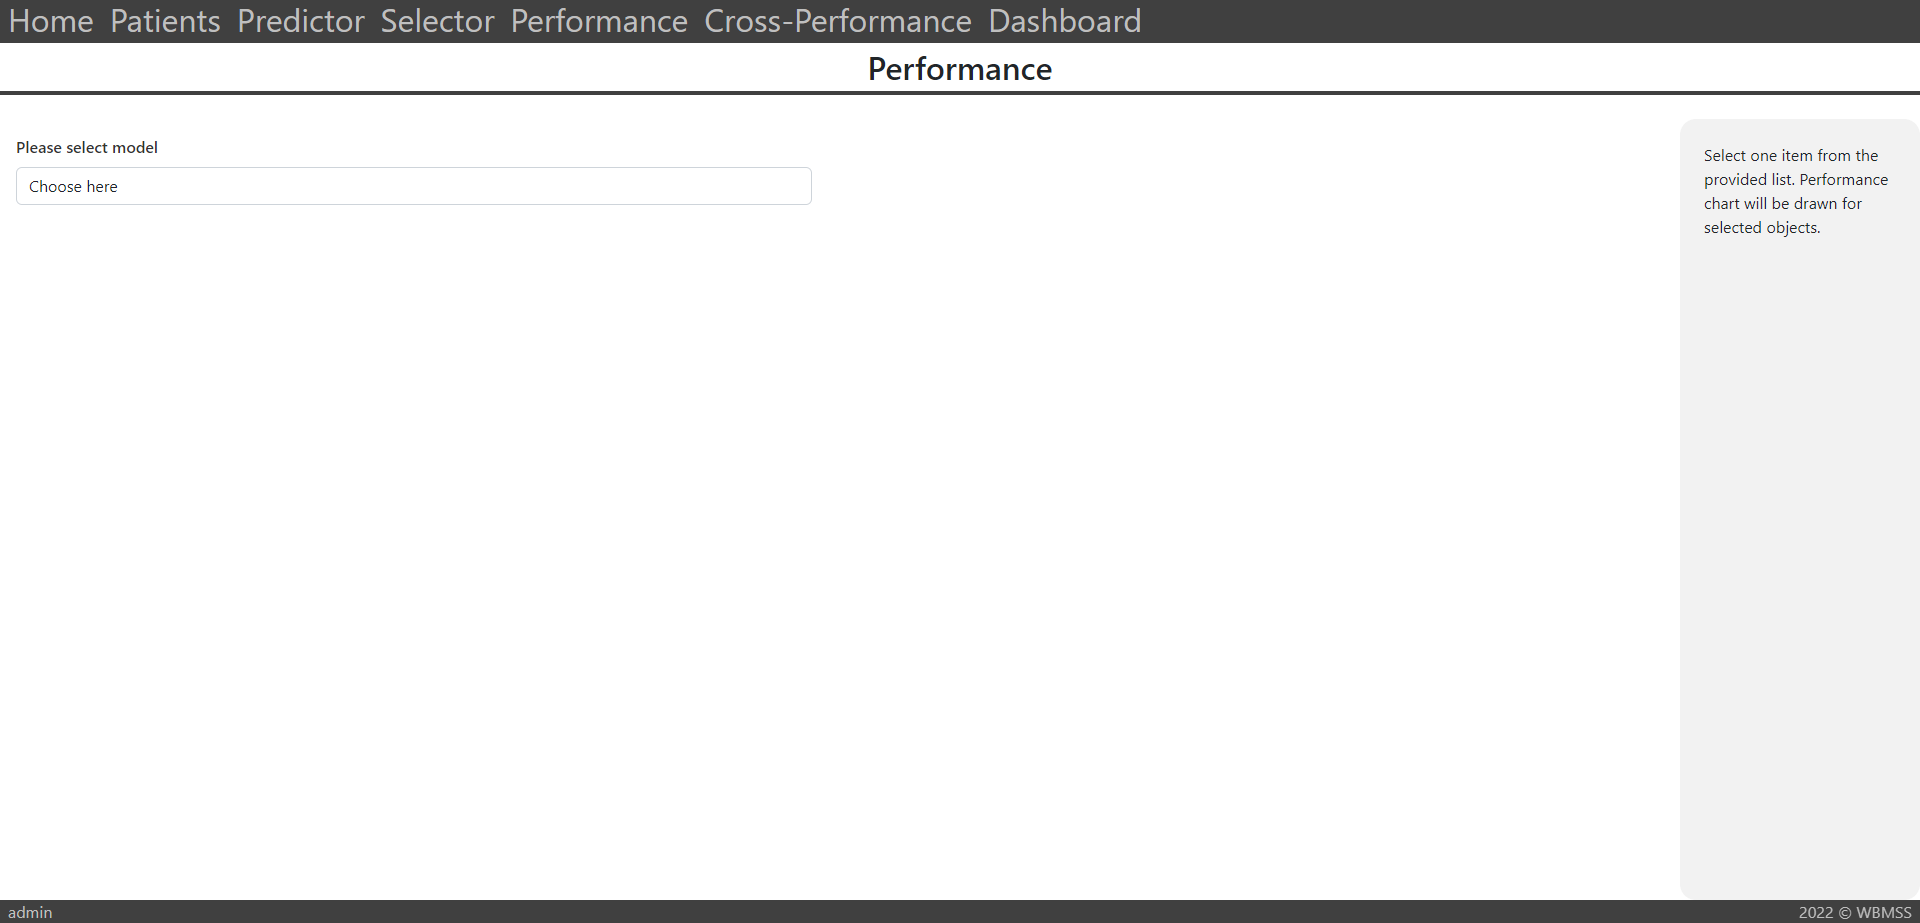
\includegraphics[width=0.7\columnwidth]{media/website/pages/performance.png}
  \caption{Performance Page}
  \label{fig:web_performance_page}
\end{figure}

\subsubsection{Performance Display Page} \label{subsubsec:performance_display_page}
This page will display the performance obtained from the performance page. This page has a similar base layout to the performance page and has an option to display the graph generated from performance. This page also acts similar to the performance page. It allows the user to select another model to display its performance. \Cref{fig:web_performance_display_page} displays the performance-display page.

\begin{figure}[H]
  \centering
  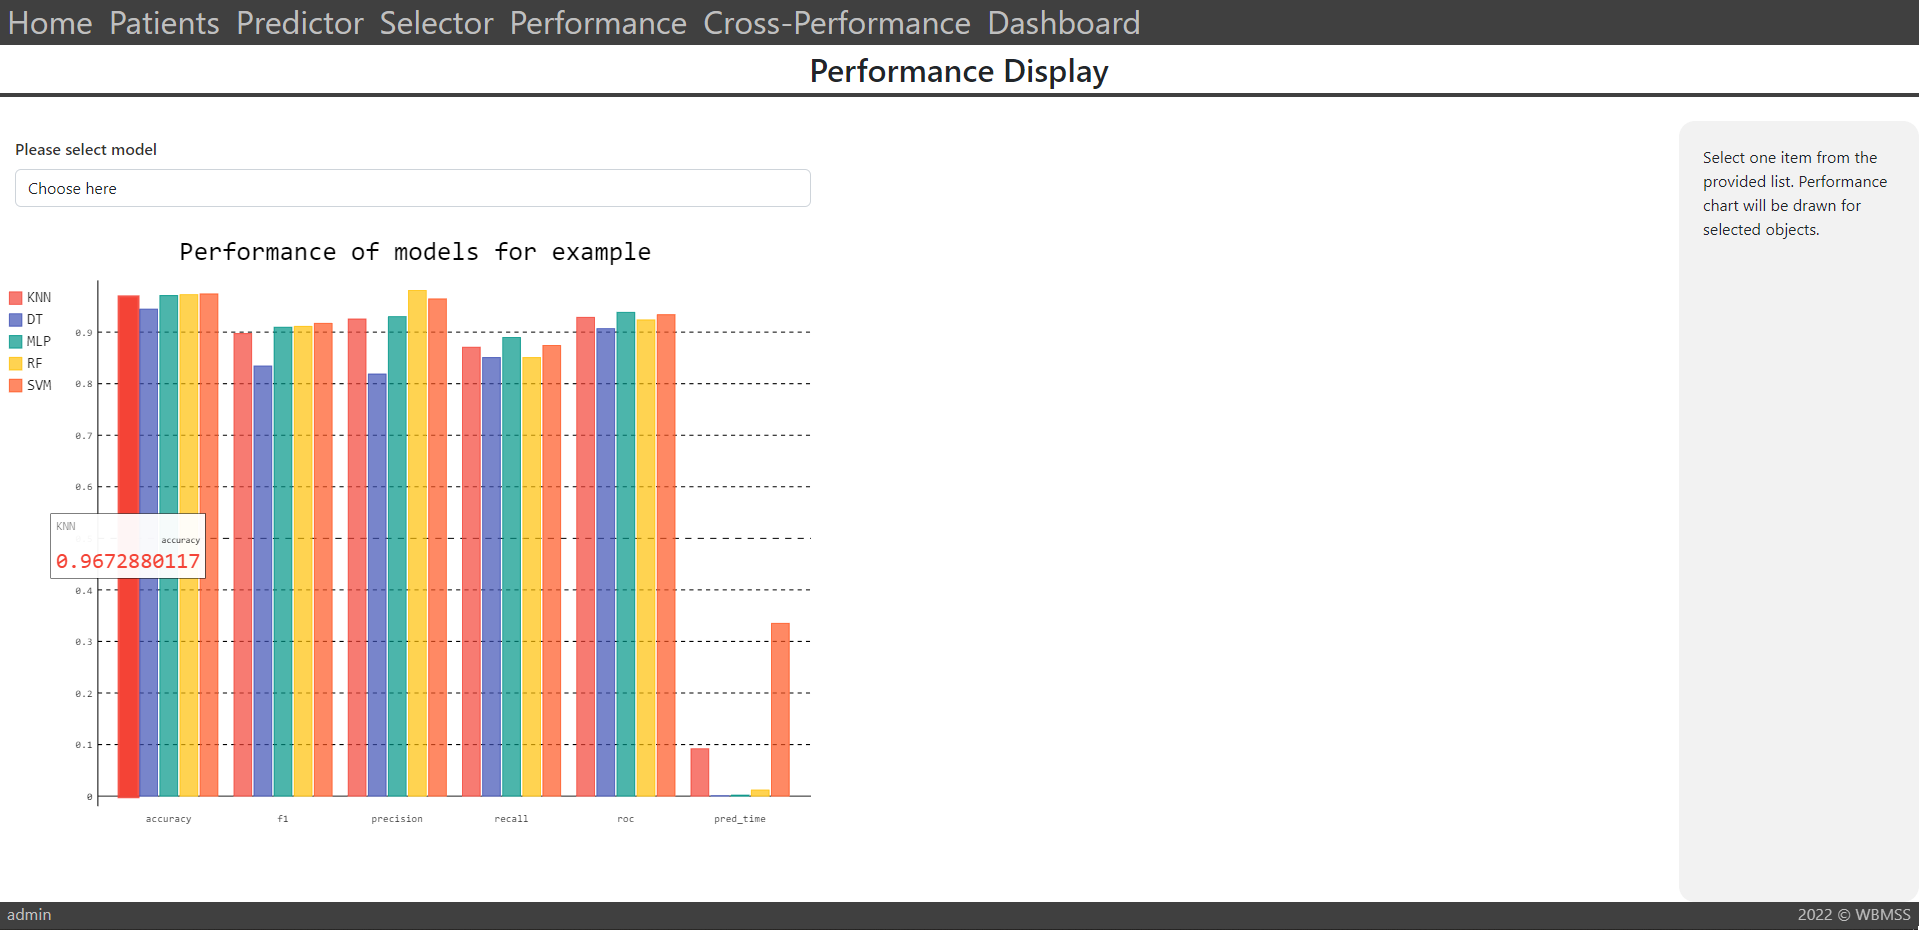
\includegraphics[width=0.7\columnwidth]{media/website/pages/performance_display.png}
  \caption{Performance Display Page}
  \label{fig:web_performance_display_page}
\end{figure}

\subsection{Cross Performance Page} \label{subsec:cross_performance_page}
This page allows users to select models from a list of models created from previous datasets. The page also provides a list of datasets uploaded by the user for predictions. The user is required to select a dataset from this list. The user-selected dataset and model will be sent to the server for cross-performance analysis. After completion of the cross-performance process, the user is redirected to the subpage. \Cref{fig:web_cross_performance_page} displays cross-performance page.

\begin{figure}[H]
  \centering
  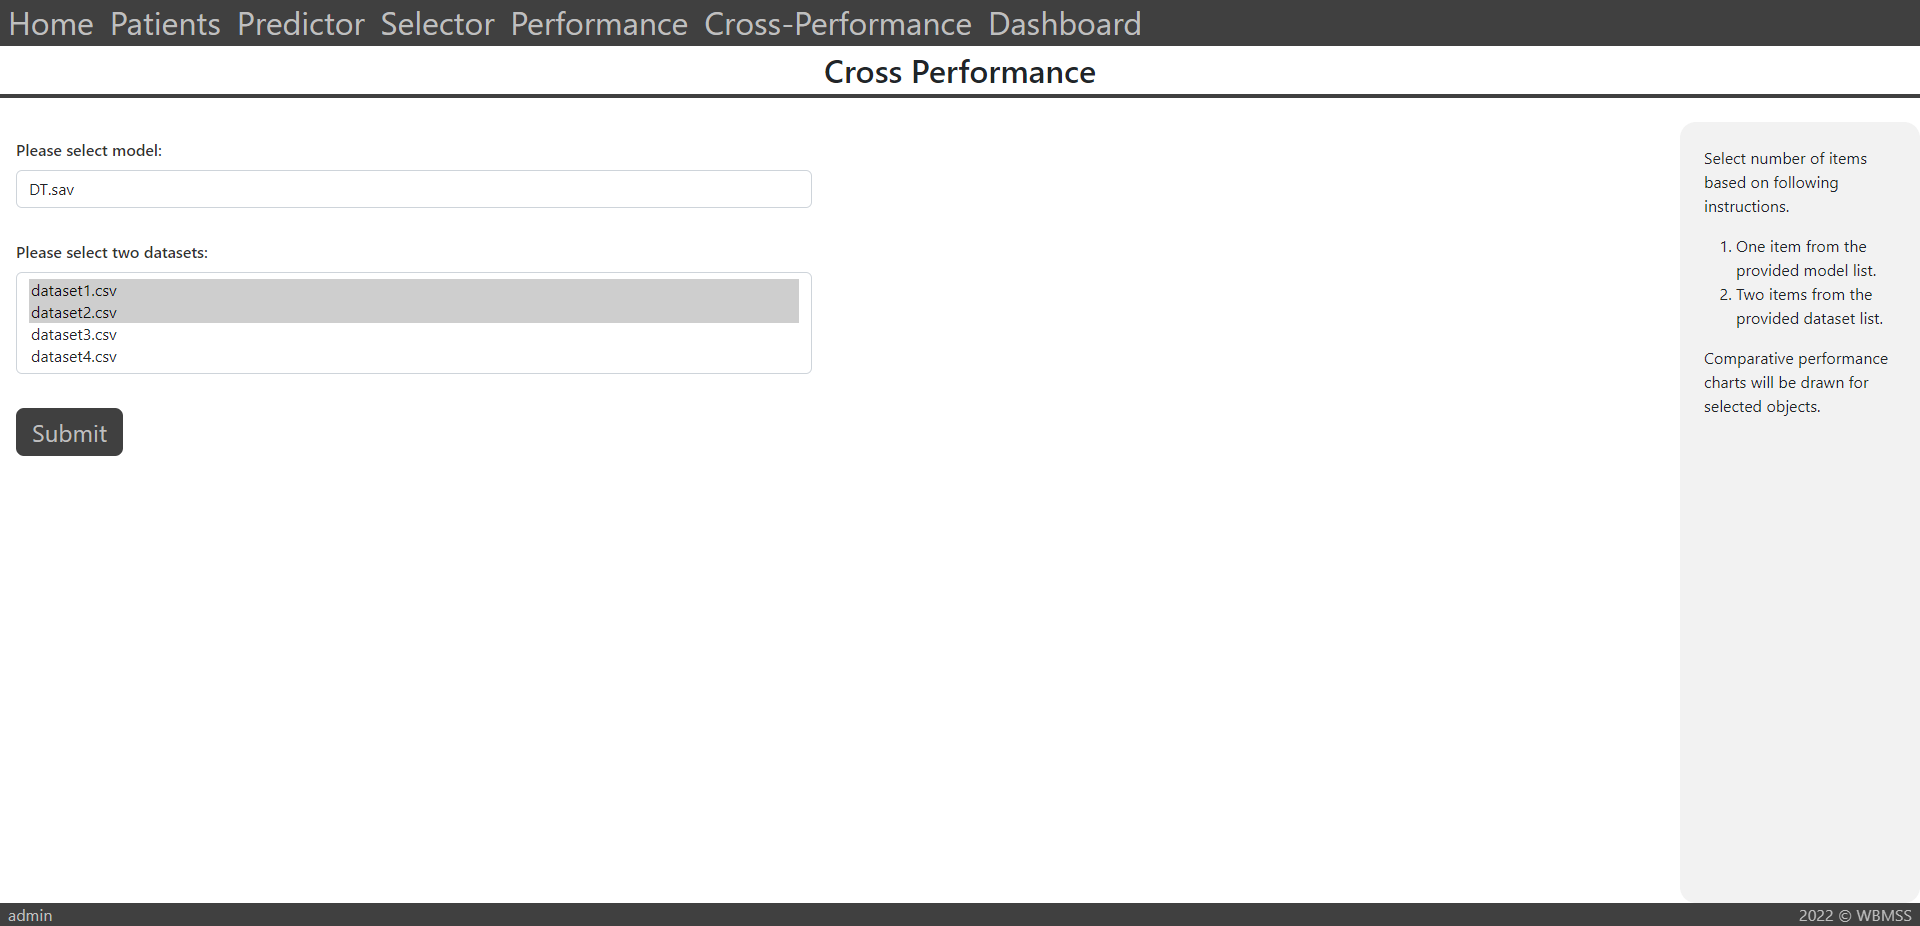
\includegraphics[width=0.7\columnwidth]{media/website/pages/cross_performance_selection.png}
  \caption{Cross Performance Page}
  \label{fig:web_cross_performance_page}
\end{figure}

\subsubsection{Cross Performance Display Page} \label{subsubsec:cross_performance_display Page} This page will receive the data obtained from the cross-performance process and display the data in chart format. This page has a similar layout and acts similar to a cross-performance page, with a display place for charts. \Cref{fig:web_cross_performance_display_page} displays the cross-performance-display page.

\begin{figure}[H]
  \centering
  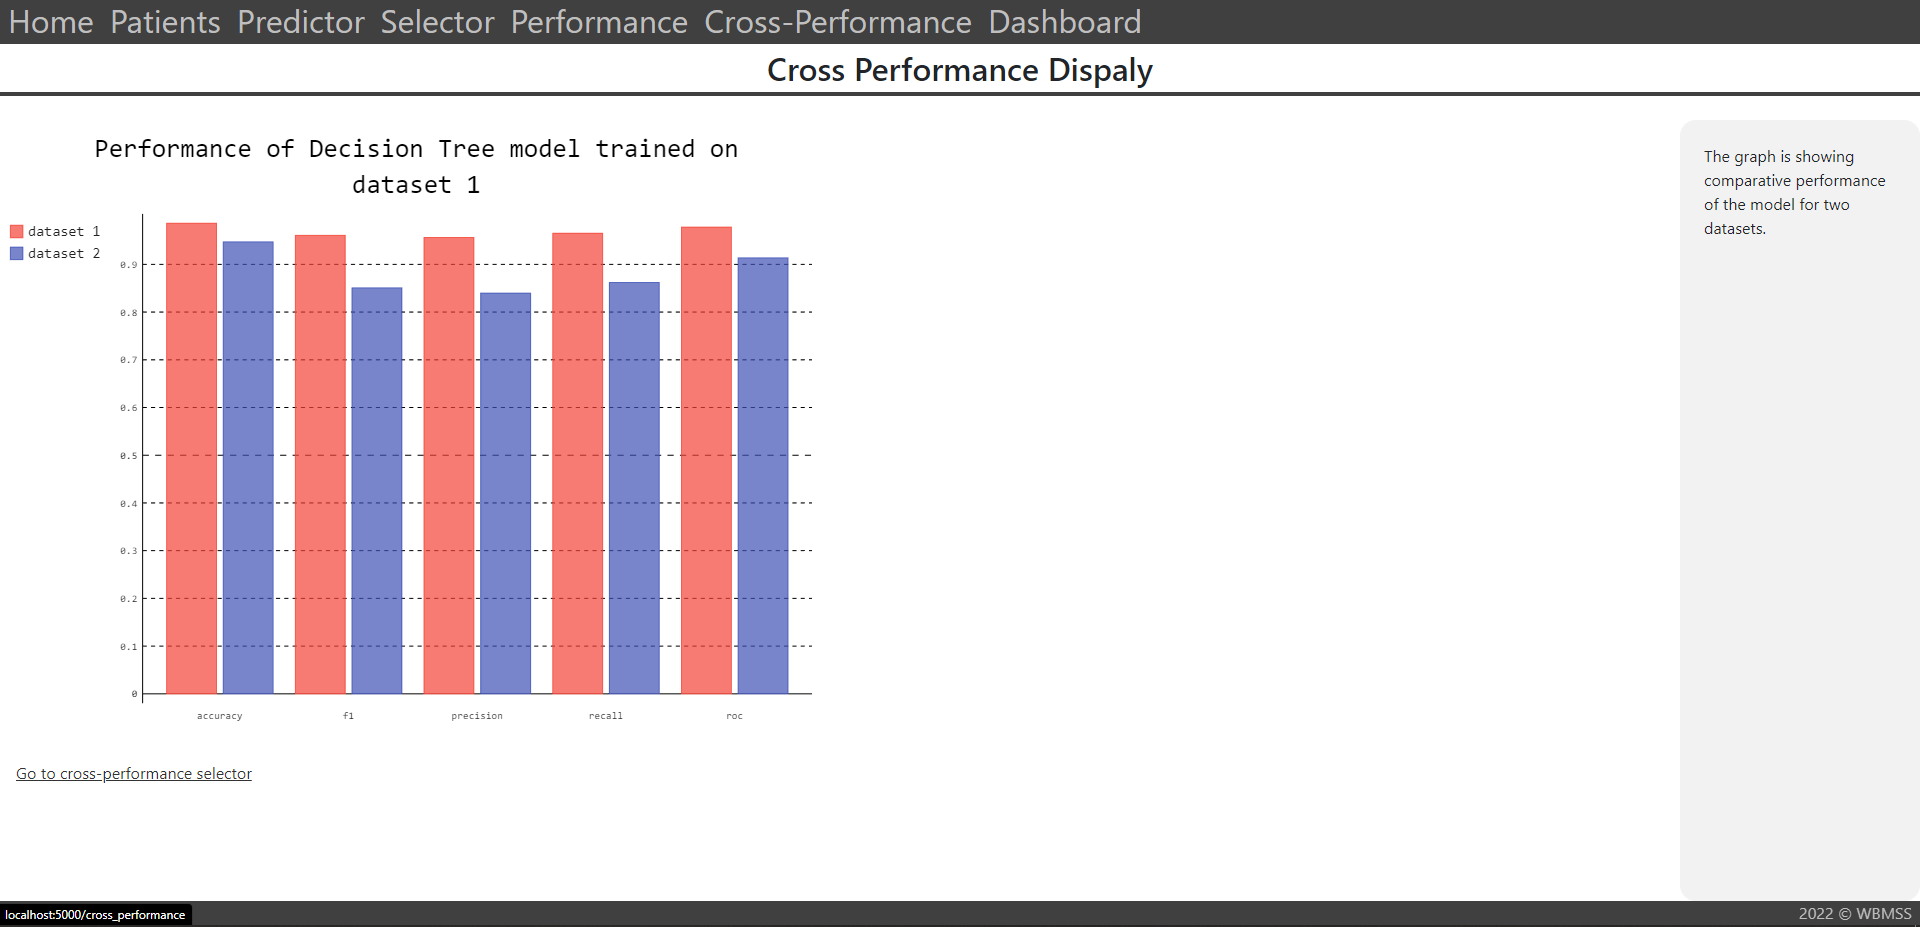
\includegraphics[width=0.7\columnwidth]{media/website/pages/cross_performance_display.png}
  \caption{Cross Performance Display Page}
  \label{fig:web_cross_performance_display_page}
\end{figure}

\FloatBarrier
\subsection{Helper Pages} \label{subsec:helper_page}
These pages act as helper pages for users as well as handles errors. In the instance of unauthorized access or invalid information, users are redirected to these pages. \Cref{fig:error_pages} shows the error pages.

\begin{figure}[H]
  \centering
  \begin{subfigure}{.7\columnwidth}
    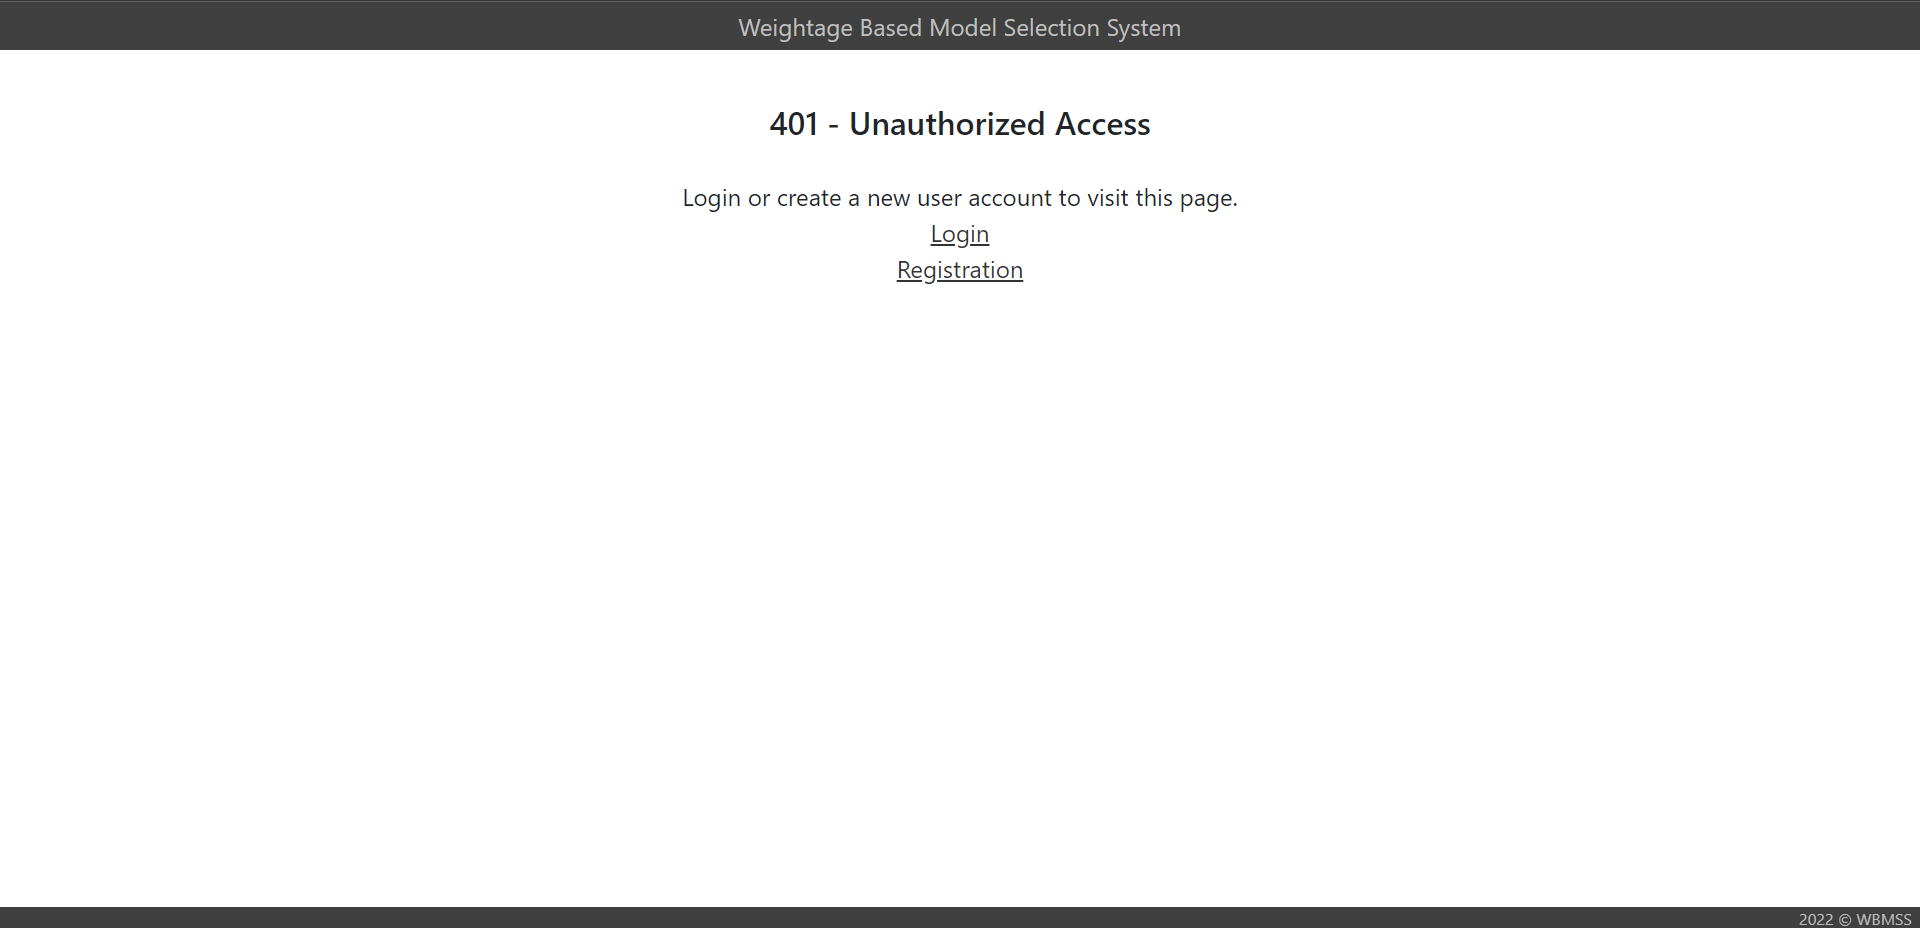
\includegraphics[width=\columnwidth]{media/website/pages/401.png}
    \caption{Unauthorized Access Error Page}
    \label{fig:401_page}
  \end{subfigure}\\
  \begin{subfigure}{.7\columnwidth}
    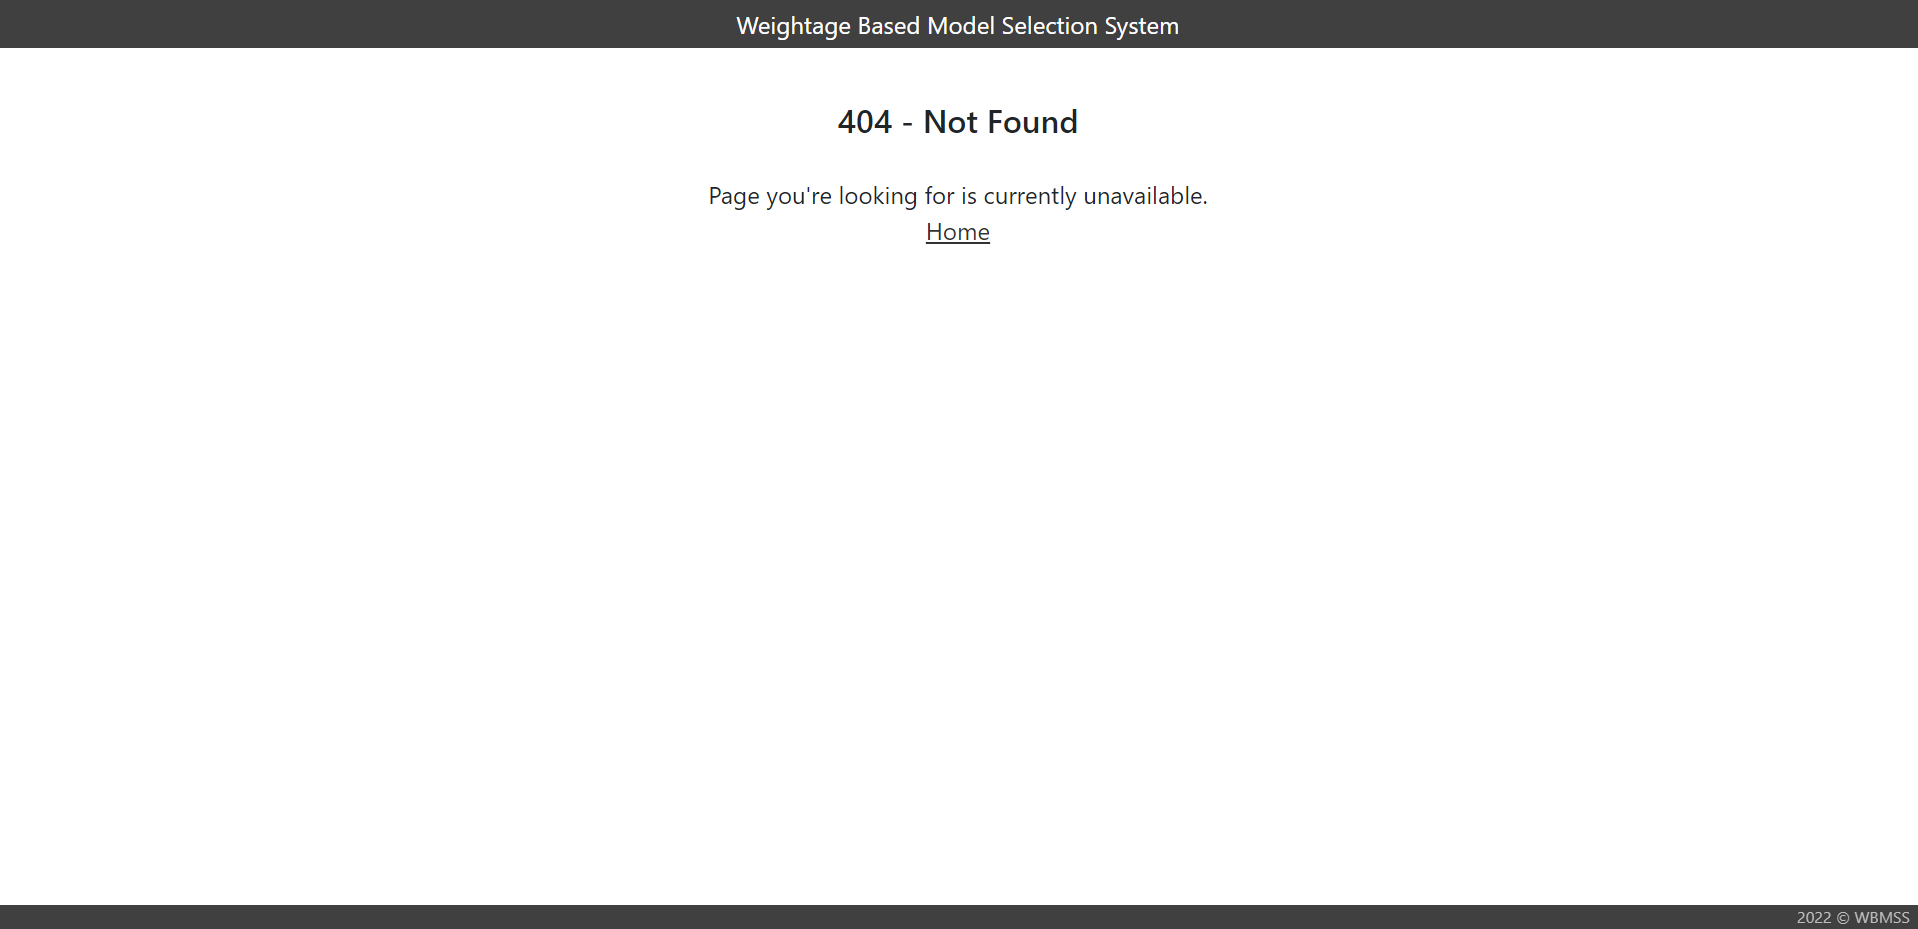
\includegraphics[width=\columnwidth]{media/website/pages/404.png}
    \caption{Not Found Error Page}
    \label{fig:404_page}
  \end{subfigure}
  \begin{subfigure}{.7\columnwidth}
    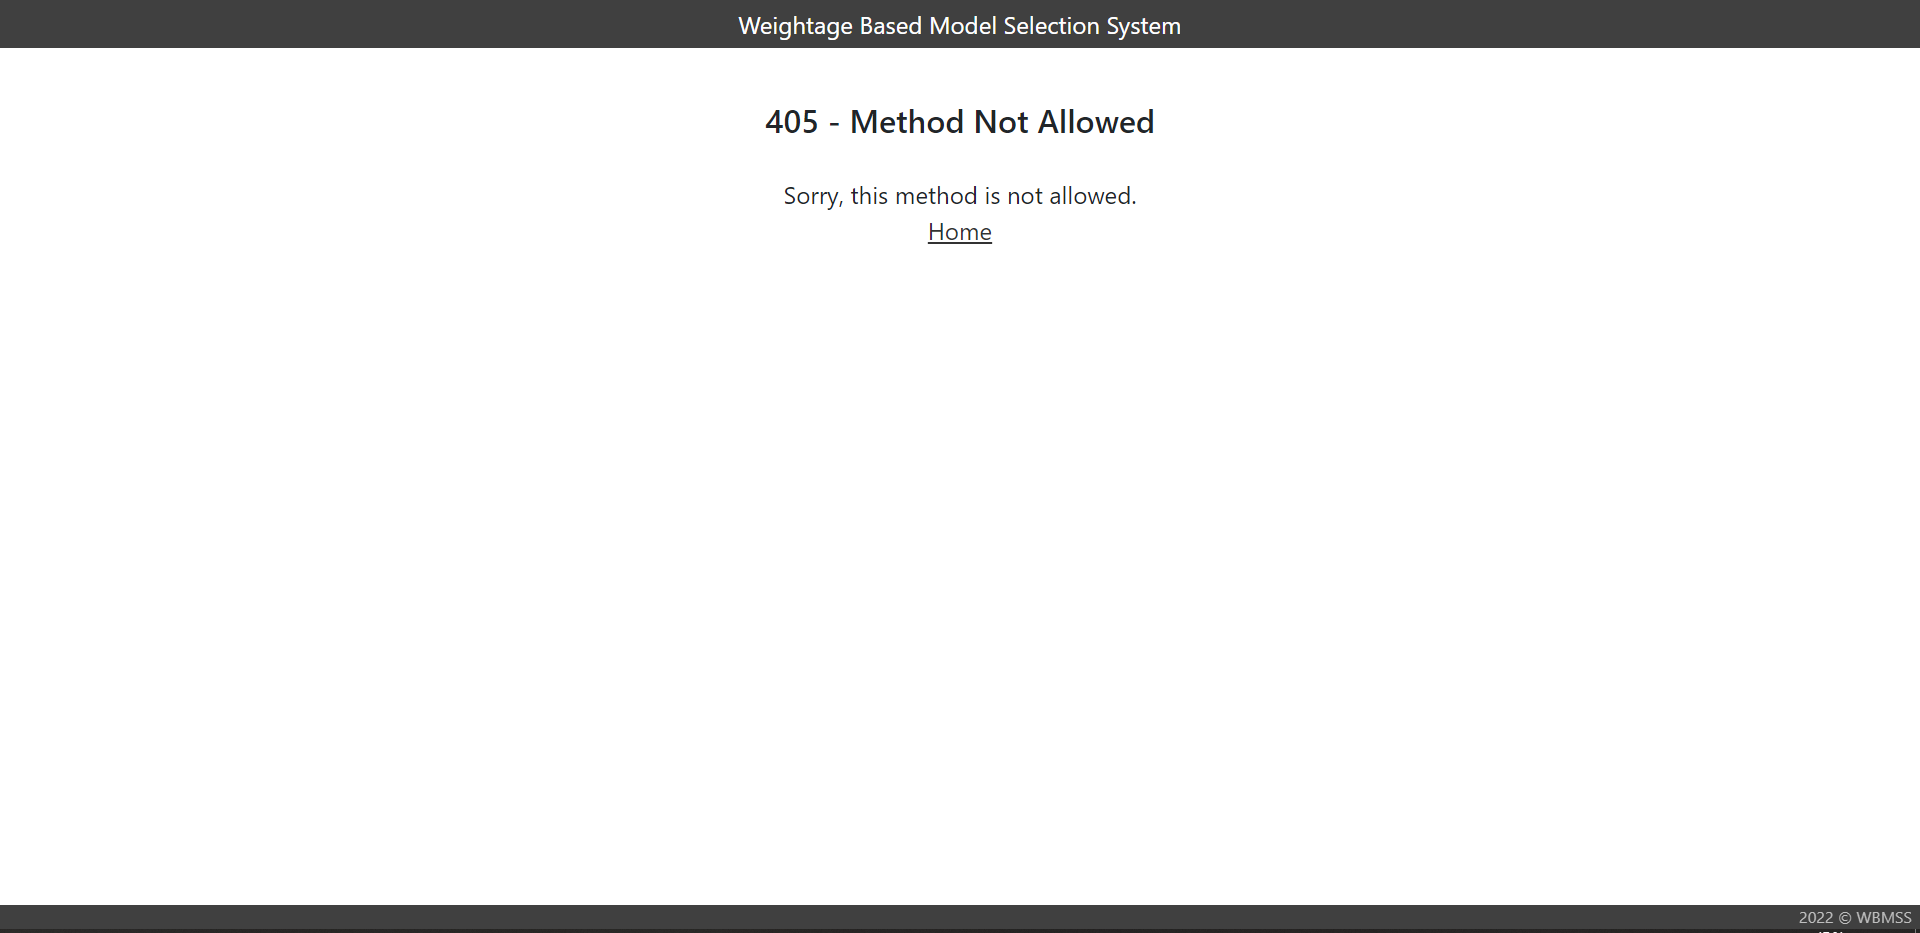
\includegraphics[width=\columnwidth]{media/website/pages/405.png}
    \caption{Method Not Allowed Page}
    \label{fig:405_page}
  \end{subfigure}%
  \caption{Error Pages}\label{fig:error_pages}
\end{figure}

\FloatBarrier
\section{Hardware Details} \label{sec:hardware_details}
The hardware used for the program is given below. The system needs at least a moderate amount of memory for operations. The amount of system memory used during development is 16 GB. The system also needs a high-performance CPU for the model training. The number of cores available for calculation is important too. The development system uses a 3.6 GHz processor with 6 Cores. The data uploaded by users and system-generated data need storage space. The recommended size of the storage is 250 GB.

Standard input and output devices are required to take data and commands from users and display them.

\begin{table}[H]
  \centering
  \caption{Hardware Details} \label{tab:hardware_details}
  \begin{tabular}{|L{10em}|L{25em}|}
    \hline
    \textbf{Hardware}      & \textbf{Details}
    \rule[-2ex]{0pt}{4ex}                                              \\\hline
    Installed memory (RAM) & 16.00 GB
    \rule[-2ex]{0pt}{4ex}                                              \\\hline
    Storage                & 250 GB SSD
    \rule[-2ex]{0pt}{4ex}                                              \\\hline
    Processor              & AMD Ryzen 5 3500 6-Core Processor 3.6 GHz
    \rule[-2ex]{0pt}{4ex}                                              \\\hline
    GPU                    & NVIDIA GeForce GTX 1650 Super
    \rule[-2ex]{0pt}{4ex}                                              \\\hline
    Input device           & Standard Keyboard and Mouse
    \rule[-2ex]{0pt}{4ex}                                              \\\hline
  \end{tabular}
\end{table}

\section{Software Details} \label{sec:software_details}
The software requirements of the application are described below. The application is developed on Windows 10 system, but it is OS independent application. The technologies used are python as a base programming language, sklearn library to make model templates, and flask to develop the web application. Pandas library is used for data handling. HTML, CSS, and JavaScript are used for web pages.

\begin{table}[H]
  \centering
  \caption{Software Requirement} \label{tab:software_requirement}
  \begin{tabular}{|L{10em}|L{25em}|}
    \hline
    \textbf{Software} & \textbf{Details}
    \rule[-3ex]{0pt}{6ex}                                                     \\\hline
    Operating System  & Windows 10
    \rule[-2ex]{0pt}{4ex}                                                     \\\hline
    Technology        & Python, Scikit-learn, Pandas, Flask, HTML, JavaScript
    \rule[-2ex]{0pt}{4ex}                                                     \\\hline
  \end{tabular}
\end{table}